\documentclass{standalone}

\usepackage{tikz}

\usetikzlibrary{positioning, chains, shapes.geometric, fit, shapes, arrows.meta, calc, backgrounds}

\begin{document}

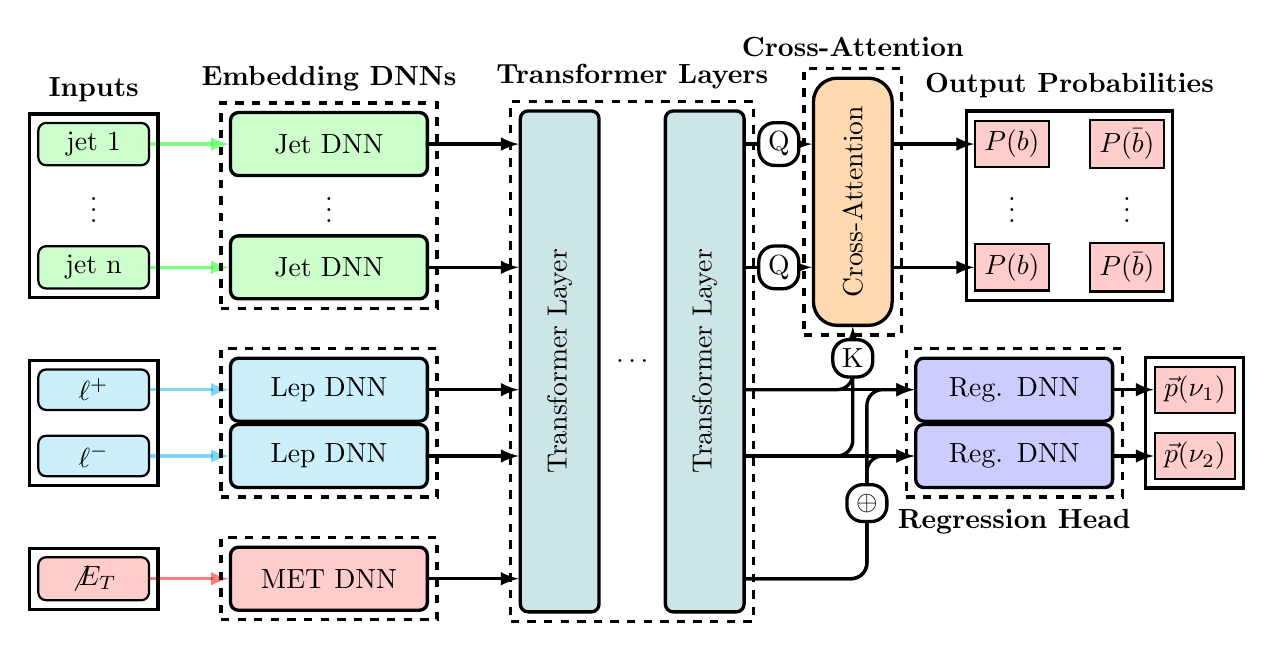
\begin{tikzpicture}[
            >=LaTeX, % Use default LaTeX arrows
            very thick,
            arrow/.style={
                        -latex,
                        very thick,
                        rounded corners=0.2cm
                  },
            block/.style={
                        rectangle,
                        fill=gray!10,
                        rounded corners=3mm,
                        draw,
                        very thick
                  },
            dnn_block/.style={
                        rectangle,
                        fill=blue!20,
                        rounded corners=1mm,
                        inner xsep=0em,
                        inner ysep=0.25em,
                        minimum height=1.4em,
                        align=center,
                        text width=2.5cm,
                        draw,
                        very thick
                  },
            transformer_layer/.style={
                        rectangle,
                        fill=teal!20,
                        rounded corners=1mm,
                        inner xsep=0em,
                        inner ysep=0.25em,
                        minimum height=1cm,
                        align=center,
                        %text width=2.5cm,
                        draw,
                        very thick
                  },
            cross_attention/.style={
                        rectangle,
                        fill=orange!30,
                        rounded corners=3mm,
                        inner xsep=1em,
                        inner ysep=1em,
                        align=center,
                        draw,
                        very thick
                  },
            input/.style={ % Input or output node
                        rectangle,
                        minimum width=4em,
                        rounded corners=1mm,
                        draw,
                        fill=green!20,
                        thick
                  },
            output/.style={ % Input or output node
                        rectangle,
                        minimum width=2.25em,
                        draw,
                        fill=red!20,
                        thick
                  }
      ]

      % Input nodes
      \node[input] (jet_1) {jet 1};
      \node[input, below=1cm of jet_1] (jet_n) {jet n};
      \node[yshift=0.05cm] at ($(jet_1)!0.5!(jet_n)$, yshift=-0.1cm) (jet_dots1) {$\vdots$};


      \node[input,fill=cyan!20, below=1cm of jet_n] (lepton_1) {$\ell^+$};
      \node[input,fill=cyan!20, below=0.3cm of lepton_1] (lepton_2) {$\ell^-$};

      \node[input,fill=red!20, below=1cm of lepton_2] (met) {$\not{E}_T$};

      % Input Embeddings for jets
      \node[dnn_block, fill=green!20,right=1cm of jet_1, minimum height = 0.8cm] (jet_dnn_1) {Jet DNN};
      \node[dnn_block, fill=green!20,right=1cm of jet_n, minimum height = 0.8cm] (jet_dnn_n) {Jet DNN};
      \node[yshift=0.05cm] at ($(jet_dnn_1)!0.5!(jet_dnn_n)$) (dnn_jet_dots) {$\vdots$};

      % Input Embeddings for leptons
      \node[dnn_block, fill=cyan!20, right=1cm of lepton_1, minimum height = 0.8cm] (lep_dnn_1) {Lep DNN};
      \node[dnn_block, fill=cyan!20, right=1cm of lepton_2, minimum height = 0.8cm] (lep_dnn_2) {Lep DNN};

      % Input Embeddings for met
      \node[dnn_block, fill=red!20,right=1cm of met, minimum height = 0.8cm] (met_dnn) {MET DNN};

      % Midpoint of the transformer layer
      \node (transformer_mid) at ($(jet_dnn_1.east)!0.5!(met_dnn.east)$) {};

      % Transformer Layers (perpendicular, rotated text)
      \path let \p1 = (jet_dnn_1.north), \p2 = (met_dnn.south) in
      node[transformer_layer,
                  right=1cm of transformer_mid,
                  minimum height={\y1-\y2},
                  minimum width=1cm]
      (transformer_1) {\rotatebox{90}{Transformer Layer}};

      \path let \p1 = (jet_dnn_1.north), \p2 = (met_dnn.south) in
      node[transformer_layer,
                  right=0.8cm of transformer_1,
                  minimum height={\y1-\y2},
                  minimum width=1cm]
      (transformer_n) {\rotatebox{90}{Transformer Layer}};

      \node at ($(transformer_1.east)!0.5!(transformer_n.west)$) (transformer_dots) {$\dots$};


      % Transformer outputs
      \node at (transformer_n.east |-  jet_1.east) (jet_1_output) {};
      \node at (transformer_n.east |-  jet_n.east) (jet_n_output) {};
      \node at (transformer_n.east |-  jet_dots1.east) (jet_dots_output) {};

      \node at (transformer_n.east |-  lepton_1.east) (lepton_1_output) {};
      \node at (transformer_n.east |-  lepton_2.east) (lepton_2_output) {};

      \node at (transformer_n.east |-  met.east) (met_output) {};

      % Cross-Attention Layer
      \path let \p1 = (jet_dnn_1.north), \p2 = (jet_dnn_n.south) in
      node[cross_attention, fill=orange!30,
                  right=0.7cm of jet_dots_output,
                  minimum height={\y1-\y2},
                  minimum width=1cm]
      (cross_attention) {\rotatebox{90}{Cross-Attention}};


      % Output Probabilities
      \node[output] at ($(cross_attention.east |- jet_1_output)+(1.5,0)$) (jet_1_prob_b) {$P(b)$};
      \node[output] at ($(cross_attention.east |- jet_n_output)+(1.5,0)$) (jet_n_prob_b) {$P(b)$};
      \node[yshift=0.05cm] at ($(jet_1_prob_b)!0.5!(jet_n_prob_b)$) (jet_prob_dots) {$\vdots$};

      \node[output, right=0.5cm of jet_1_prob_b] (jet_1_prob_bbar) {$P(\bar{b})$};
      \node[output, right=0.5cm  of jet_n_prob_b] (jet_n_prob_bbar) {$P(\bar{b})$};
      \node[yshift=0.05cm] at ($(jet_1_prob_bbar)!0.5!(jet_n_prob_bbar)$) (output_bbar_dots) {$\vdots$};

      % Regression DNN
      \node[dnn_block, right=2cm of lepton_1_output, minimum height = 0.8cm] (lepton_1_reg) {Reg. DNN};
      \node[dnn_block, right=2cm of lepton_2_output,minimum height = 0.8cm] (lepton_2_reg) {Reg. DNN};

      % Regression Output
      \node[output, right=0.5cm of lepton_1_reg] (lepton_1_reg_output) {$\vec{p}(\nu_1)$};
      \node[output, right=0.5cm of lepton_2_reg] (lepton_2_reg_output) {$\vec{p}(\nu_2)$};





      % Boxes around groups of nodes
      \node[fit=(jet_1)(jet_n),
      draw,
      inner sep=0.1cm,
      label=above:{\textbf{Inputs}}]
      (input_box) {};

      \node[fit=(lepton_1)(lepton_2),
            draw,
            inner sep=0.1cm]
      (input_box) {};

      \node[fit=(met),
            draw,
            inner sep=0.1cm]
      (input_box) {};

      % Jet embeddings
      \node[fit=(jet_dnn_1)(jet_dnn_n),
      draw,
      dashed,
      inner sep=0.1cm,
      label=above:{\textbf{Embedding DNNs}}]
      (embedding_box) {};

      % Lepton and MET embeddings
      \node[fit=(lep_dnn_1)(lep_dnn_2),
            draw,
            dashed,
            inner sep=0.1cm,
      ]
      (lepton_met_embedding_box) {};

      \node[fit=(met_dnn),
            draw,
            dashed,
            inner sep=0.1cm]
      (met_embedding_box) {};

      % Transformer layers
      \node[fit=(transformer_1)(transformer_n),
      draw,
      dashed,
      inner sep=0.1cm,
      label=above:{\textbf{Transformer Layers}}]
      (transformer_box) {};

      % Cross-Attention layer
      \node[fit=(cross_attention),
      draw,
      dashed,
      inner sep=0.1cm,
      label=above:{\textbf{Cross-Attention}}]
      (cross_attention_box) {};

      % Output probabilities
      \node[fit=(jet_1_prob_b)(jet_n_prob_b)(jet_1_prob_bbar)(jet_n_prob_bbar),
      draw,
      inner sep=0.1cm,
      label=above:{\textbf{Output Probabilities}}]
      (output_box) {};

      % Regression DNNs
      \node[fit=(lepton_1_reg)(lepton_2_reg),
      draw,
      dashed,
      inner sep=0.1cm,
      label=below:{\textbf{Regression Head}}]
      (regression_box) {};

      % Regression outputs
      \node[fit=(lepton_1_reg_output)(lepton_2_reg_output),
            draw,      inner sep=0.1cm,]
      (regression_output_box) {};

      % Draw arrows between layers
      % Arrows from inputs to embeddings
      \draw[arrow, color=green, opacity=0.5, blend mode=multiply] (jet_1) -- (jet_dnn_1);
      \draw[arrow,color=green, opacity=0.5, blend mode=multiply] (jet_n) -- (jet_dnn_n);
      \draw[arrow, color=cyan, opacity=0.5, blend mode=multiply] (lepton_1) -- (lep_dnn_1);
      \draw[arrow, color=cyan, opacity=0.5, blend mode=multiply] (lepton_2) -- (lep_dnn_2);
      \draw[arrow, color=red, opacity=0.5, blend mode=multiply] (met) -- (met_dnn);

      % Arrows from embeddings to transformer
      \draw[arrow] (jet_dnn_1.east) -- (transformer_1.west |- jet_dnn_1.east);
      \draw[arrow] (jet_dnn_n.east) -- (transformer_1.west |- jet_dnn_n.east);
      \draw[arrow] (lep_dnn_1.east) -- (transformer_1.west |- lep_dnn_1.east);
      \draw[arrow] (lep_dnn_2.east) -- (transformer_1.west |- lep_dnn_2.east);
      \draw[arrow] (met_dnn.east) -- (transformer_1.west |- met_dnn.east);

      % Arrows from transformer to cross-attention
      \draw[arrow](jet_dnn_1.east -| transformer_n.east) -- (jet_dnn_1.east -| cross_attention.west) node[midway, fill=white, draw, rectangle] {Q};
      \draw[arrow] (jet_dnn_n.east -| transformer_n.east) -- (jet_dnn_n.east -| cross_attention.west)  node[midway, fill=white, draw, rectangle] {Q};

      \draw[arrow] (lep_dnn_2.east -| transformer_n.east) -|  ( cross_attention.south);
      \draw[arrow] (lep_dnn_1.east -| transformer_n.east) -|  ( cross_attention.south) node[near end, fill=white, draw, rectangle] {K};

      % Arrows from cross-attention to outputs
      \draw[arrow] (cross_attention.east |- jet_1_output) -- (jet_1_prob_b.west);
      \draw[arrow] (cross_attention.east |- jet_n_output) -- (jet_n_prob_b.west);


      % Arrows from transformer to regression DNNs
      \draw[arrow] (lep_dnn_2.east -| transformer_n.east) -- (lepton_2_reg.west);
      \draw[arrow] (lep_dnn_1.east -| transformer_n.east) -- (lepton_1_reg.west);

      \draw[arrow] (met_dnn.east -| transformer_n.east) -|  ($(lepton_2_reg.west)+(-0.6,0)$) --  (lepton_2_reg.west);

      \draw[arrow] (met_dnn.east -| transformer_n.east) -| node[pos=0.7, fill=white, draw, rectangle] {$\oplus$} ($(lepton_1_reg.west)+(-0.6,0)$) --  (lepton_1_reg.west);


      % Arrows from regression DNNs to regression outputs
      \draw[arrow] (lepton_1_reg.east) -- (lepton_1_reg_output.west);
      \draw[arrow] (lepton_2_reg.east) -- (lepton_2_reg_output.west);


\end{tikzpicture}
\end{document}